%%%% CAPÍTULO 2 - REVISÃO DA LITERATURA (OU REVISÃO BIBLIOGRÁFICA, ESTADO DA ARTE, ESTADO DO CONHECIMENTO)
%%
%% O autor deve registrar seu conhecimento sobre a literatura básica do assunto, discutindo e comentando a informação já publicada.
%% A revisão deve ser apresentada, preferencialmente, em ordem cronológica e por blocos de assunto, procurando mostrar a evolução do tema.
%% Título e rótulo de capítulo (rótulos não devem conter caracteres especiais, acentuados ou cedilha)
\chapter{Referencial te\'orico}\label{cap:referencialTeorico}

Neste capítulo será discorrido sobre os principais conceitos que justificam o escopo deste trabalho, como o que são e qual a importância dos SIEMs na área de segurança da informação, o que são as regras \textit{Sigma}, o que são LLMs e como os assuntos se relacionam entre si.

\section{Segurança da Informação e SOC}



\subsection{SIEM}

Um Sistema de Gerenciamento de Informações e Eventos de Segurança, do inglês \textit{Security Information and Event Management} (SIEM) funciona como o núcleo central de inteligência em ambientes de cibersegurança,
agregando e correlacionando \textit{logs} provindos de toda a infraestrutura de TI --- como \textit{firewalls}, sistemas de detecção de intrusão (IDS), todos os tipos de servidores, bancos de dados e entre outras inúmeras aplicações. 
Sua essência reside na capacidade de contextualizar eventos aparentemente desconexos, identificando padrões que ferramentas isoladas não detectariam. 
Conforme destacam \citeonline{PodzinsRomanovs}, essa contextualização é crucial em ações automatizadas contra ameaças complexas e citam o exemplo de um ataque de \textit{zero-day}, onde a correlação entre uma tentativa de força bruta no \textit{Active Directory} 
(serviço de diretório da \textit{Microsoft} que gerencia identidades, recursos e permissões dentro da rede interna) e a existência de tráfego suspeito no \textit{firewall} pode disparar respostas imediatas.

Nos Centros de Operações de Segurança (SOCs), o SIEM assume um papel operacional indispensável. 
Ele consolida alertas de diferentes fontes e formatos, prioriza incidentes com base na criticidade e orquestra processos de resposta (\textit{workflows}). 
\citeonline{PodzinsRomanovs} enfatizam ainda que, sem um SIEM, os SOCs perdem a capacidade de detectar fases avançadas de ataques, como por exemplo, de movimento lateral e escalação de privilégios, que se caracterizam pela movimentação do invasor por meio dos sistemas do alvo enquanto adquire privilégios de acesso ---visando o nível de administrador; 
é citado o caso da rede de hoteis \textit{Starwood}, que permaneceu quatro anos sem identificar uma violação sequer e sofreu um vazamento de dados de 383 milhões de hóspedes ao redor do mundo em 2019 \cite{Marriot}. 
Diante do exposto, essa visão unificada transforma o SIEM no ``sistema nervoso'' do SOC, permitindo que analistas investiguem ameaças sistêmicas, não apenas alertas isolados. 

A eficácia de um SOC está intrinsecamente ligada à maturidade do SIEM. 
Regras mal calibradas geram excesso de falsos positivos; 
SIEMs não otimizados podem produzir mais de mil alertas diários, sobrecarregando as equipes --- segundo \citeonline{PodzinsRomanovs}, uma pessoa sozinha é capaz de analisar apenas cerca de 5 a 15 alertas por dia, a depender da criticidade dos mesmos. 
Por outro lado, uma configuração refinada permite que um único analista investigue milhares de \textit{logs}, elevando exponencialmente a eficiência operacional. 
A empresa Exabeam reforça que essa otimização é a base para um SOC ágil e proativo \cite{Exabeam1}.

A importância estratégica de um SIEM convencional na cibersegurança moderna se ancora na sua capacidade de reduzir drasticamente o tempo de detecção de ameaças, principalmente porque, conforme o passar dos anos, qualquer tipo de dado se tornou o recurso mais valioso que existe. 
\citeonline{PodzinsRomanovs} citam um relatório de vazamentos de dados de 2018 da Verizon \cite{verizon2018dbir}, informando que cerca de 68\% das violações são descobertas meses (ou mais) após o ataque inicial; 
o último relatório, de 2025, não atualiza esta porcentagem, mas informa que o tempo médio de remediação de vulnerabilidades nos dispositivos de borda (especialmente falhas de \textit{zero-day}) é de 32 dias \cite{verizon2025dbir}. 
Este tipo de lacuna pode ser preenchida quando se tem um SIEM bem implementado, em virtude da correlação dos eventos em tempo real. 
Além disso, ele serve como alicerce para a evolução tecnológica: plataformas SIEM convencionais são a base necessária para a integração de IA e aprendizado de máquina, que posteriormente amplificam a detecção de ameaças sutis e permitem a automação de respostas \cite{PaloAlto1}.

>>>>Qual a diferença entre um SIEM e um antivírus tipo o Acronis?<<<<<<<<

Economicamente, embora o SIEM convencional envolva custos elevados (licenças baseadas em volume de \textit{logs}, equipe especializada e SOC ininterrupto), \citeonline{PodzinsRomanovs} justificam seu investimento frente ao cenário de riscos globais: projetou-se US\$ 5,2 trilhões em perdas por ciberataques entre 2019 –- 2023. 
Para organizações com dados sensíveis ou requisitos de conformidade, como o GDPR --- Regulamento Geral sobre a Proteção de Dados da União Europeia, ou a PCI-DSS --- \textit{Payment Card Industry Data Security Standard}, norma globalmente reconhecida aplicada à segurança de dados de cartões de pagamento, o SIEM é não apenas viável, mas indispensável;
sua ausência representa um lapso operacional intransponível, mesmo com outras soluções de segurança.

Em suma, o SIEM convencional se mantém como pilar irrevogável da segurança corporativa; 
não por sua tecnologia isolada, mas também por habilitar ecossistemas integrados de detecção e resposta. 
Conclui-se que sua implementação estratégica, ainda que desafiadora, é um divisor de águas entre organizações expostas a violações prolongadas e aquelas capazes de antecipar, conter e remediar ameaças em escala evolutiva.


\subsection{SIEMs Inteligentes}

A integração de aprendizado de máquina (do inglês, \textit{machine learning}, ML) e inteligência artificial (IA) em SIEMs transforma a cibersegurança ao superar as limitações das abordagens baseadas em regras estáticas. 
De acordo com \citeonline{Saddi2024}, a IA generativa consegue criar dados sintéticos para simular ameaças inéditas, permitindo a detecção proativa de ataques \textit{zero-day} sem depender exclusivamente de dados previamente rotulados. 
Essa capacidade é amplificada pelos algoritmos de ML que analisam padrões contextuais em grandes volumes de \textit{logs}, correlacionam eventos aparentemente desconexos (como tráfego anômalo com tentativas de força bruta) e identificam ameaças complexas. 
A predição de ameaças e a automatização dessas análises são fatores críticos para a atuação dos SOCs.

A integração de técnicas de IA e aprendizado de máquina em sistemas SIEM melhora significativamente a correlação de grandes volumes de eventos em tempo real, reduzindo falsos positivos ou falsos negativos, acelerando a triagem de alertas \cite{PaloAlto1}.
Conforme demonstrado por \citeonline{Nurusheva2024}, algoritmos de detecção de anomalias, análise preditiva e limiares adaptativos permitem identificar proativamente atividades sutis ou ocultas que escapariam sob regras estáticas ou análise manual. 
Ainda, ao empregar ambos modelos supervisionados e não supervisionados, o SIEM com ML aprende continuamente a partir dos dados de \textit{logs} e do comportamento da rede, ajustando-se dinamicamente às mudanças no ambiente e antecipando novos vetores de ataque \cite{jordan2015machine}.

É visto que, com o crescimento exponencial de dados e o aumento da complexidade das ameaças, é inviável depender exclusivamente de analistas humanos, tornando substancial o uso estratégico de ML/IA por parte dos SIEMs.
Essa prática permite que o SIEM evolua de uma abordagem baseada em regras para uma abordagem comportamental e baseada em risco, onde perfis de usuários e entidades são criados automaticamente e usados para detectar desvios. 
Isso se alinha com o trabalho de \citeonline{Saddi2024}, que propõem modelos de IA generativa para analisar fluxos de dados e gerar respostas simuladas a possíveis ataques, ajudando a antecipar e mitigar riscos de forma mais eficaz. 
Portanto, a incorporação de IA e ML em SIEMs representa um avanço significativo para a cibersegurança moderna, trazendo precisão, adaptabilidade e automação a um cenário cada vez mais dinâmico e hostil.


\section{Bases de Padrões de Ataques}

Para a criação de regras em SIEMs, assim como para qualquer tipo de regra, há de se adotar algum padrão.
No mundo da cibersegurança existem padrões que catalogam e identificam vulnerabilidades, eventos e outras categorias do gênero. 
Duas categorizações são o CVE e o CWE.
O CVE --- \textit{Common Vulnerabilities and Exposures} (Vulnerabilidades e Exposições Comuns), é um programa mantido pelo MITRE desde 1999, que define e cataloga vulnerabilidades e exposições de segurança publicamente conhecidas, no qual se atribui um identificador único (CVE-ID) e padrão para cada uma.
Atualmente possuindo quase 300 mil registros, o CVE é uma referência confiável para integrar bancos de dados de segurança, alertas, produtos comerciais e soluções automatizadas \cite{NIST_CVE_Process, CVE_History}.

Já o CWE --- \textit{Common Weakness Enumeration} (Enumeração de Fraquezas Comuns), também mantido pelo MITRE, é um catálogo comunitário de tipos de fraquezas (como falhas de validação, \textit{buffer overflow}, injeção), usadas para identificar a causa raiz subjacente às vulnerabilidades. 
Quando um CVE descreve um ``\textit{buffer overflow}'', ele pode ser correlacionado a um CWE específico, permitindo que os analistas entendam quando se trata de um erro de lógica, design ou implementação \cite{CWE_About, CWE_Usage_Guidance}.

O MITRE, que mantém as duas listagens citadas acima, é uma organização sem fins lucrativos, mantida por agências como o NIST (Instituto Nacional de Padrões e Tecnologia, do inglês \textit{National Institute of Standards and Technology}) 
e CISA (Agência de Segurança Cibernética e Infraestrutura, do inglês \textit{Cybersecurity and Infrastructure Security Agency}). 
Além da contribuição citada acima, o MITRE criou uma solução alternativa chamada MITRE ATT\&CK --- 
uma base de dados sobre táticas e técnicas adversárias, acessível globalmente, baseada em observações do mundo real. 
É usada como base para o desenvolvimento de modelos e metodologias de ameaças no setor privado, governo e na comunidade de produtos e serviços de cibersegurança \cite{MITRE_ATTACK}.
A base é aberta e está disponível gratuitamente para uso de qualquer indivíduo ou organização, assim como o CVE e CWE. 

Não menos importante é o NVD --- \textit{National Vulnerability Database} ou Base Nacional de Dados de Vulnerabilidades, repositório do governo dos EUA e mantido pelo NIST.
É responsável por armazenar dados padronizados sobre vulnerabilidades de segurança seguindo o protocolo SCAP (\textit{Security Content Automation Protocol}. 
O repositório inclui listas de falhas em \textit{softwares}, métricas de impacto, nomes de produtos, configurações vulneráveis e \textit{checklists}, permitindo automação da gestão de vulnerabilidades, avaliação de segurança e conformidade \cite{NIST_NVD_General}. 

Esses elementos são pilares para as regras de SIEMs/\textit{Sigma}, pois fornecem contexto de acionamento e padronização. 
O NVD enriquece CVEs com dados de severidades (como o CVSS (\textit{Common Vulnerability Scoring System}), método usado para fornecer uma medida qualitativa de gravidade \cite{NIST_NVD_Metrics})
e produtos afetados, permitindo que SIEMs priorizem alertas com base no risco real. 
As classificações CWE ajudam a desenvolver regras \textit{Sigma} para fraquezas comuns, detectando ataques mesmo quando variantes novas surgem.
Já o mapeamento MITRE entre CWE e CVE vincula falhas de código a vulnerabilidades exploradas, refinando a correlação de ameaças em SIEMs. 
Por exemplo, uma regra \textit{Sigma} pode usar o CWE-352\footnote{Falsificação de solicitação entre sites, do inglês \textit{Cross-Site Request Forgery} (CSRF) \cite{CWE_352}.} 
para monitorar solicitações não autorizadas, enquanto o CVE associado direciona \textit{patches} críticos \cite{nist_cwe_slice}.

\section{Regras \textit{Sigma}}

Sigma (\textit{Generic Signature Format for SIEM Systems}, ``Assinatura em formato genérico para sistemas SIEM'' em tradução livre \cite{SigmaReadMe}) 
é o projeto de código aberto de um padrão genérico de descrição de \textit{logs} de eventos, aplicável a qualquer tipo de \textit{log},
com o intuito de compartilhar a lógica de detecção de ameaças ou anomalias entre diferentes SIEMs. 
Ao operar com dados de ameaças de múltiplas fontes, o \textit{Sigma} capacita os caçadores de ameaças a correlacionar eventos que passariam despercebidos por abordagens convencionais. 
Dessa forma, se obtém conhecimentos estratégicos sobre dados confiáveis e antecipa-se tentativas de ataque em estágios iniciais desta cadeia de eventos \cite{Splunk1}.

Os mantenedores da iniciativa consideram que excelentes análises podem ser encontradas na \textit{internet}, incluindo IOCs e regras YARA\footnote{Uma regra YARA é um arquivo de extensão ``.yar'' contido de expressões lógicas usadas para classificar e identificar amostras de \textit{malware} \cite{PicusSecurity}.} para detectar arquivos ou ferramentas maliciosos, por exemplo, mas que muitas vezes limitam-se a descrições específicas, funcionais para poucos \textit{softwares}.
Portanto, da necessidade de haver um método de descrição específico ou genérico de eventos de \textit{logs}, com portabilidade para vários SIEMs, a fim de aprimorar os recursos de detecção para todos, surgiu o Sigma \cite{SigmaReadMe}.

O projeto de código aberto foi criado em 2017 por Florian Roth e Thomas Patzke \cite{AboutSigma}, inspirados em padrões já existentes nas áreas de análise de \textit{malware} e monitoramento de rede. Como já dito, o padrão \textit{Sigma} se diferencia por lidar com vários tipos de esquemas de \textit{logs}, unindo padrões que já existem e se diferenciam entre si \cite{Splunk1}. 

O projeto carrega essa denominação pois se considera um ecossistema --- envolve três componentes: o formato \textit{Sigma}, a ferramenta \textit{Sigma} e a coleção de regras \textit{Sigma}. 
Este último diz respeito ao repositório no \textit{Github}, que possui mais de 3 mil regras de detecção de diferentes tipos; 
por ser de código aberto, pode receber sugestões de qualquer pessoa disposta a contribuir \cite{SigmaReadMe}. 
Já a ferramenta \textit{Sigma}, refere-se a um conversor de regras disponível para \textit{download} --- o \textit{Sigma Command Line Interface} (CLI). 
Com ele é possível converter as regras \textit{Sigma} para as regras usadas no SIEM de interesse do usuário; 
\textit{Elasticsearch}, \textit{CrowdStrike}, \textit{IBM QRadar AQL} e \textit{Splunk} são algumas marcas registradas para as quais essa integração está disponível.

\subsection{Sigma e a mitigação de ameaças}

As regras \textit{Sigma} formam um conjunto estruturado de princípios e métodos essenciais para o sucesso da investigação focada em determinar as ameaças que podem prejudicar um ou mais sistemas (\textit{Threat Hunting}), 
oferecendo um padrão uniforme que orienta os profissionais de segurança na elaboração de regras criteriosas para detecção de ameaças ou anomalias. 
Segundo \citeonline{Dimitrov2025YARA}, essas regras otimizam a identificação, avaliação e a resposta a incidentes,
proporcionando decisões mais precisas e oportunas, além de uma base sólida para controlar vetores de ameaças, minimizar riscos e prevenir violações de dados.
Dessa forma, as regras \textit{Sigma} constituem o alicerce de uma estratégia de segurança proativa e resiliente, capaz de antecipar e mitigar possíveis ataques de forma sustentável.

A caça a ameaças é um processo defensivo proativo que visa descobrir e neutralizar invasores, mapeando vulnerabilidades e antecipando movimentos adversos por meio da análise contínua de comportamentos anômalos e incidentes em curso.
Nesse cenário, as regras \textit{Sigma}, desde sua padronização, em 2017, desempenham um papel fundamental ao oferecer uma linguagem comum para correlação de eventos em múltiplas plataformas SIEM,
unificando dados de sistemas heterogêneos e acelerando a detecção de padrões suspeitos.
Conforme demonstrado por \citeonline{Dimitrov2025YARA}, essa unificação reduz significativamente a carga de trabalho manual dos analistas, 
permitindo identificar ameaças ainda na fase inicial de comprometimento, elevando a eficácia das operações de \textit{Threat Hunting}, ou ``caça a ameaças''.

No entanto, ainda que a aplicação das regras \textit{Sigma} viabilize inúmeros cenários benquistos, vale ressaltar que, ainda assim, os SIEMs continuarão sendo heterogêneos, pois utilizam formatos e padrões de dados diferentes --- situação inclusive de eventos de diferentes dispositivos. 
As regras \textit{Sigma} surgem como uma forma de expressar a regra ou a ameaça e o que deve ser buscado, mas ainda precisa ser convertida para o SIEM de destino (através do CLI), que já possui suas próprias regras.

\subsection{Estrutura}

As regras \textit{Sigma} são arquivos YAML contidos de informações que viabilizam a detecção de comportamento estranho ou malicioso quando da inspeção de arquivos de \textit{logs} dentro do contexto de um SIEM \cite{SigmaRules}. 

A compreensão da estrutura de uma regra \textit{Sigma} e como é usada para detecção faz-se importante em razão de que parte da metodologia envolverá selecionar as informações mais críticas das regras e avaliá-las.

As regras são divididas em três grupos principais de instruções \cite{SigmaRules}: 
\begin{itemize}
    \item Detecção (\textit{detection}): qual comportamento malicioso a regra está procurando;
	\item Fonte do log (\textit{logsource}): quais tipos de logs a detecção deve procurar; e
    \item Metadados (\textit{title}, \textit{id}, \textit{status}, etc.): detalhes da regra. 
\end{itemize}

A Figura \ref{fig:figura1} é um exemplo de regra \textit{Sigma} que está disponível na página oficial do projeto.  

\begin{figure}[htb]
    \caption{Exemplo de regra \textit{Sigma} \cite{SigmaRules}} 
	\label{fig:figura1}
    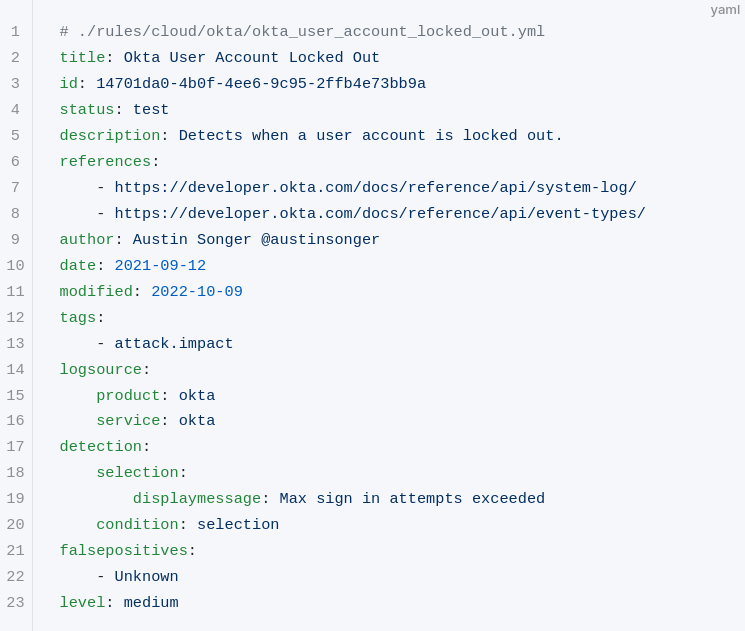
\includegraphics[scale=0.45]{figuras/figura 1.png}
	\fonte{Captura de tela da página \textit{Sigma Rules} em \citeonline{SigmaRules}}%% Fonte
\end{figure}

A seção de detecção é o coração da regra \textit{Sigma}, pois especifica o alvo da regra no vasto volume de \textit{logs}. 
Adiante neste trabalho este componente será mencionado como um dos principais para a análise da qualidade das regras geradas pelas IAs. 
Vale mencionar que, dentro da seção de detecção, existem instruções para a escrita, assim como qualquer linguagem de programação; 
no entanto, num primeiro momento, basta compreender o esqueleto principal. 
Sendo assim, a segunda peça mais importante da regra é a fonte dos \textit{logs}, o campo \textit{logsource}; 
nele se especifica qual o tipo de \textit{log} deve ser canalizado pela regra --- ao invés de varrer todos os \textit{logs} do SIEM. 
Por fim, as demais informações, os metadados, servem para guiar o usuário sobre o assunto da regra \cite{SigmaRules}. 

Para fins de orientação quando da criação de uma nova regra, é disponibilizado um esqueleto da regra com instruções (Figura \ref{fig:figura2}) no repositório \textit{Sigma} \cite{RuleCreationGuide}. 

\begin{figure}[htb]
    \caption{Exemplo de regra \textit{Sigma} \cite{RuleCreationGuide}} 
	\label{fig:figura2}
    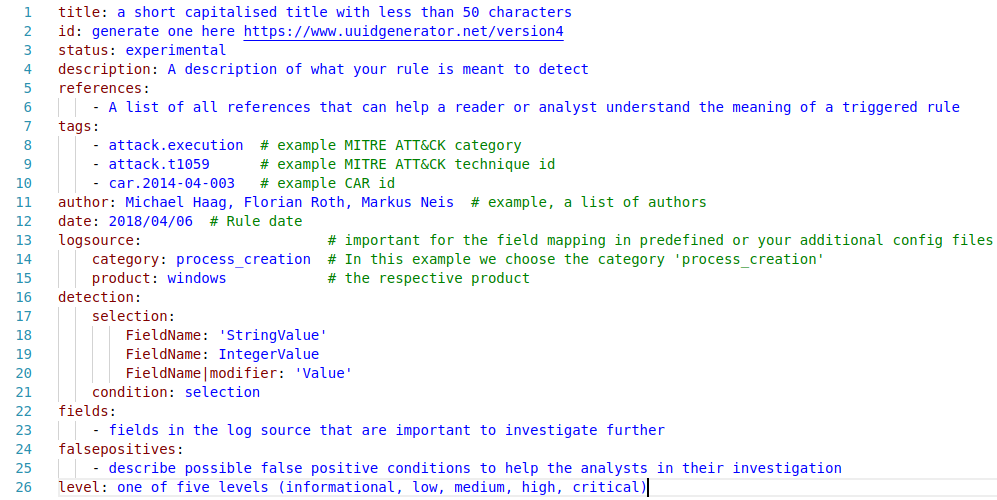
\includegraphics[scale=0.45]{figuras/figura 2.png}
	\fonte{Captura de tela do código genérico na página \textit{Rule Creation Guide} no repositório Sigma\cite{RuleCreationGuide}}%% Fonte
\end{figure}
    

\section{Processamento de Linguagem Natural}

Segundo \citeonline{liddy2001natural}, o Processamento de Linguagem Natural (PLN) é definido como uma abordagem computacional teórica e tecnológica fundamentada para analisar textos em linguagem humana. 
Seu objetivo central é alcançar um processamento linguístico semelhante ao humano, através da representação de textos aos níveis linguísticos:  
fonológico (padrões de entonação e fonemas), morfológico (estrutura das palavras), léxico (significado individual das palavras), sintático (estrutura gramatical das frases), semântico (significado literal das frases), discursivo (coesão e estrutura dos textos) e pragmático (contexto);
ou seja, o PLN fragmenta o texto e analisa sistematicamente as sete camadas citadas \cite{liddy2001natural, Chowdhary2020}.

As técnicas de PLN evoluíram de métodos simbólicos, baseados em regras e lógica formal, para abordagens estatísticas e conexionistas (ou seja,  inspirada no funcionamento do cérebro humano),
impulsionadas pelos avanços computacionais e a disponibilidade de coleções extensas e estruturadas de textos \cite{liddy2001natural}.

O PLN suporta aplicações críticas como a Recuperação de Informação (RI), Extração de Informação (EI), Tradução Automática (TA) e Sistemas de Pergunta-Resposta. 
\citeonline{liddy2001natural} cita um exemplo de RI em que sistemas PLN melhoraram a precisão em representar consultas e documentos em diversos níveis semânticos.
A EI utiliza reconhecimento de entidades e análise parcial para estruturar dados de textos não estruturados, como em anúncio de emprego.
Já os sistemas de diálogo, embora ainda dependentes de dimensões fonético-léxicas, buscam incorporar todas as camadas linguísticas para resultados mais naturais.
A sumarização automatizada --- geração de resumos concisos e coerentes a partir de textos extensos, aplica análise discursiva para condensar os textos enquanto mantém coerência \cite{Chowdhary2020, liddy2001natural}.

Alguns dos obstáculos do PLN envolvem a integração de conhecimento de mundo e raciocínio de senso comum, essenciais para resolver ambiguidades contextuais complexas.
Avanços nos modelos híbridos e ferramentas aceleram os experimentos, mas a compreensão profunda permanece distante, pois exige bases de conhecimento amplas e técnicas como inferência abdutiva para superar lacunas de interpretação \cite{Chowdhary2020}. 


\subsection{Modelos de Linguagem de Grande Escala (LLMs)}

Os Grandes Modelos de Lingugagem, do inglês \textit{Large Language Models} (LLMs),
são sistemas de inteligência artificial treinados com bilhões ou trilhões de parâmetros,
capazes de compreender e gerar textos em linguagem natural, ou seja, no formato de comunicação humano.
A arquitetura desses modelos é baseada em ``\textit{Transformers}'' --- redes neurais baseadas em mecanismos de \textit{self-attention} 
que permitem que o modelo foque em diferentes partes do texto simultaneamente, adquirindo relações contextuais de longo alcance entre as palavras \cite{weber2024redpajamaopendatasettraining};  
estes aprendem em grande escala através do aprendizado auto supervisionado (\textit{self-supervised learning}), extraindo padrões de grandes corpos de textos sem rótulos explícitos \cite{hasanov2024application}.
A evolução dessas redes marca um avanço na capacidade das máquinas ``entenderem'' contexto e intenção.

>>>>>>>>>>>>>>>>>>>>\citeonline{motlagh2024llmcyber} explica que o mecanismo central de um LLM se baseia na predição de \textit{tokens} (menores unidades de texto que um modelo de linguagem divide para processar) sequenciais: 
dada uma sequência de entrada, o modelo estima a probabilidade do próximo elemento textual, refinando essa habilidade ao longo do pré-treino.
Além disso, explica que técnicas como a ``\textit{in-context learning}'' permitem que o mesmo modelo execute tarefas específicas apenas com os exemplos fornecidos pelo \textit{prompt}, sem haver necessidade de ajuste fino. 
Esse paradigma torna possível a aplicação do mesmo modelo de LLM em diferentes tarefas sem precisar retreiná-lo \cite{motlagh2024llmcyber}.

>>>>>>>>>>>>>>>>>>>>>A aplicabilidade dos LLMs é vasta: auxiliam na geração de código, criação de conteúdos, atendimento ao cliente, análise de sentimentos e suporte à decisão clínica, entre outras funções \cite{motlagh2024llmcyber}. 
Contudo, desafios sempre existirão, e o alto custo computacional é um deles, além da tendência de reprodução de vieses presentes nos dados originais e vulnerabilidade a ataques de \textit{jailbreak}\footnote{Processo de exploração de falhas de um dispositivo eletrônico bloqueado para instalar outro \textit{software} que não o disponibilizado pelo fabricante para uso no dispositivo \cite{kaspersky2024jailbreaking}.}
e injeção de \textit{prompt}\footnote{Ocorre quando \textit{prompts} do usuário alteram o comportamento ou a saída do LLM de maneiras não intencionais. 
Essas entradas podem afetar o modelo mesmo que sejam imperceptíveis para humanos. Portanto, as injeções de \textit{prompt} não precisam ser visíveis/legíveis para humanos, desde que o conteúdo seja analisado pelo modelo. \cite{owasp2024promptinjection}}.
Superar qualquer entrave exigirá trabalho contínuo, transparência dos dados e aperfeiçoamento incessante das técnicas de mitigação de riscos. 


\subsection{Arquitetura Transformer}



\subsection{Engenharia de Prompt}



\section{Geração Aumentada por Recuperação (RAG)}



\subsection{\textit{Embeddings} e Bancos de Dados Vetoriais}



\subsection{RAG aplicado à Cibersegurança}



\section{Agentes Autônomos}



%\subsection{Padrão ReAct}



\subsection{LangGraph como Orquestrador}